\documentclass{standalone}
\usepackage{tikz}
\usetikzlibrary{patterns, positioning}
\usepackage[sfdefault]{ClearSans} %% option 'sfdefault' activates Clear Sans as the default text font
\usepackage[T1]{fontenc}

\begin{document}
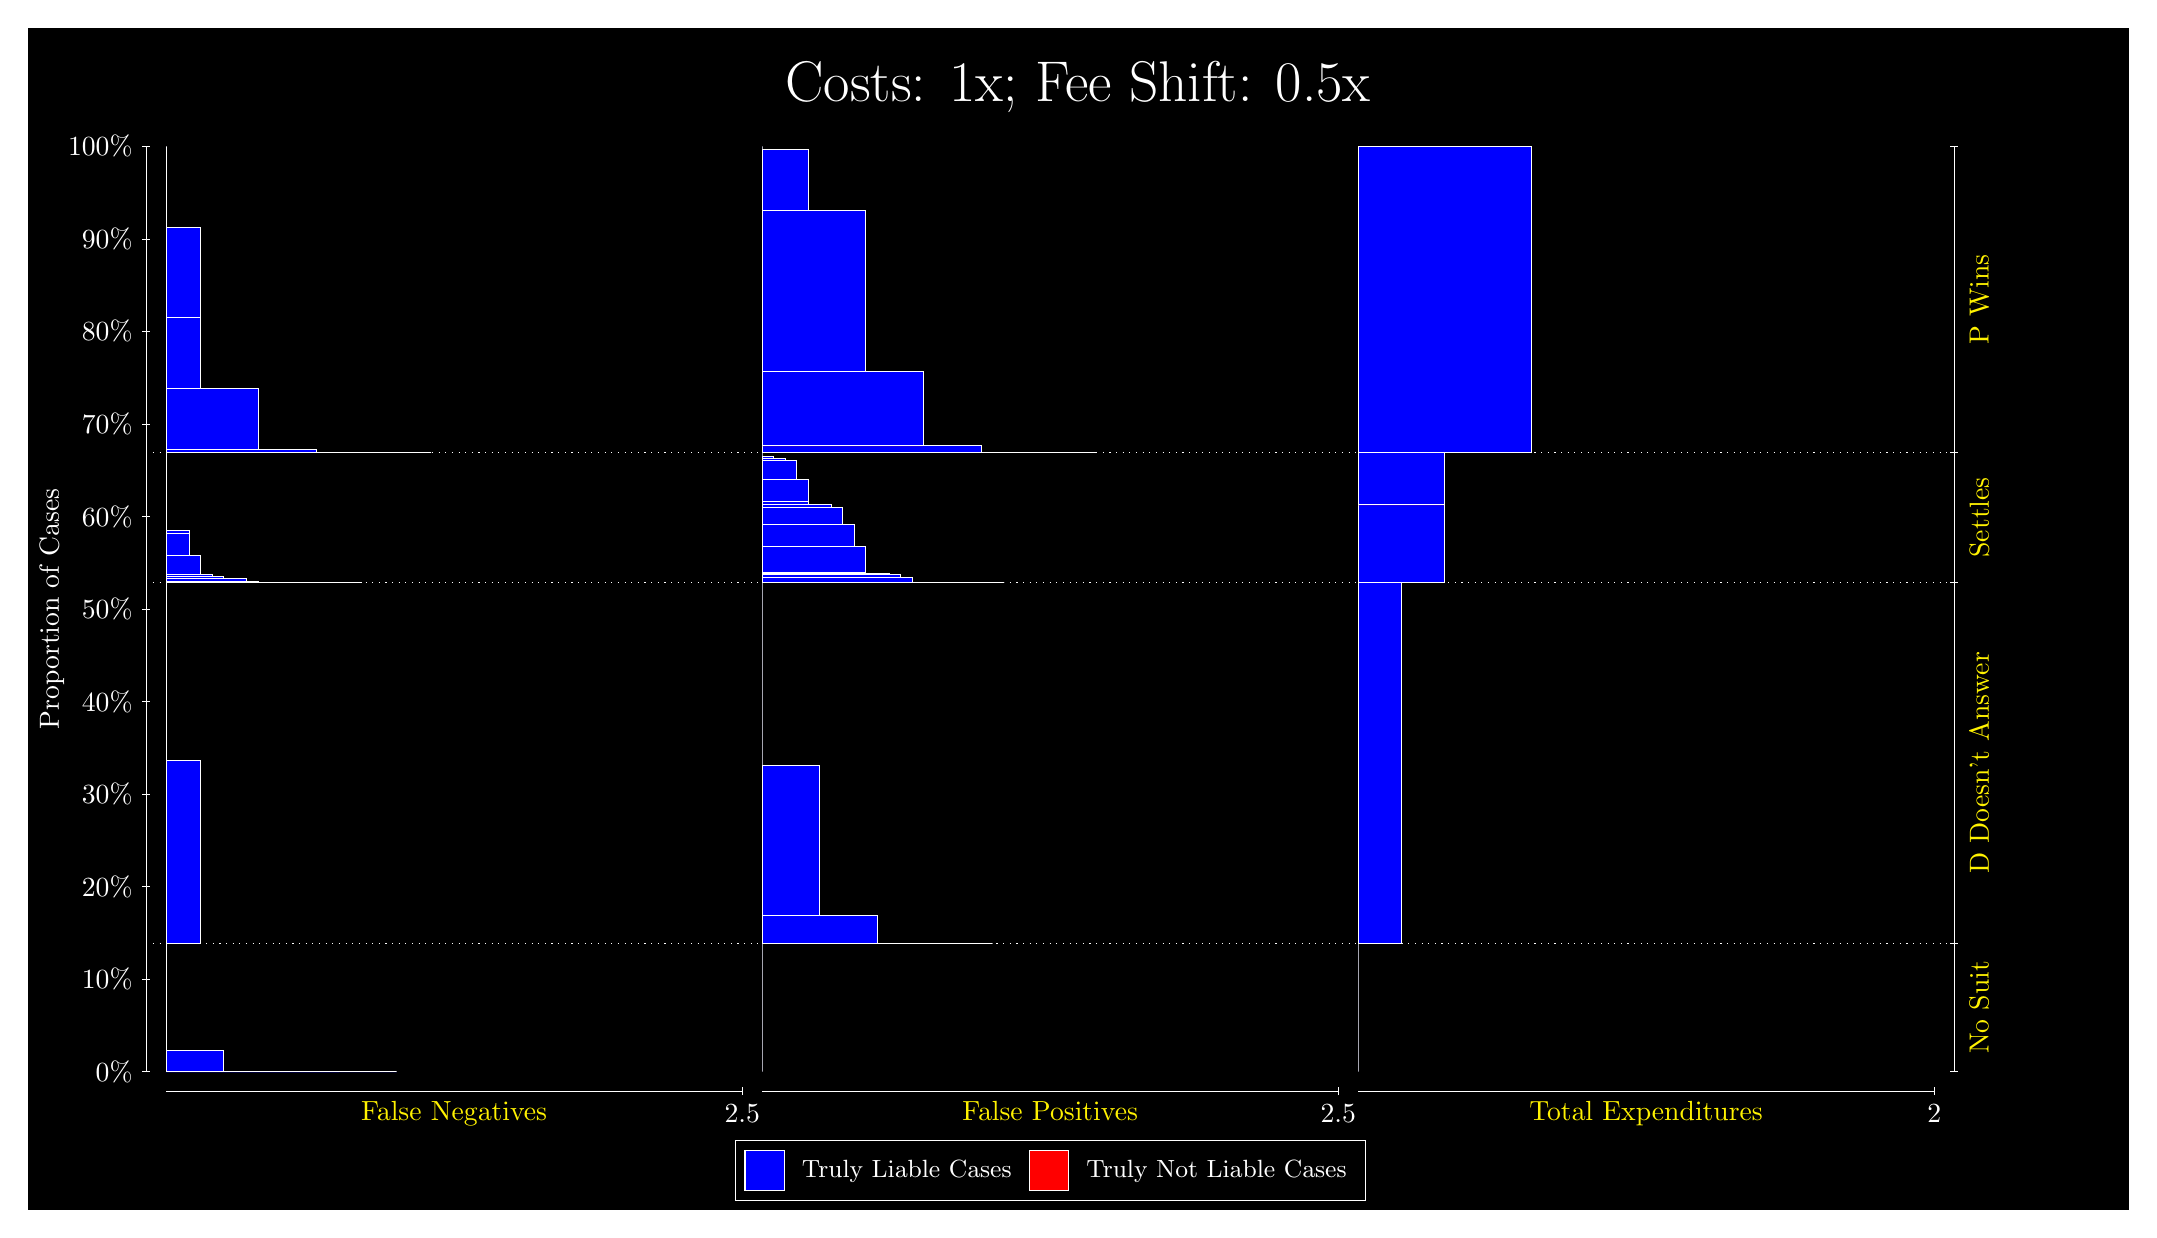
\begin{tikzpicture}
\draw[fill=black] (0,0) rectangle (26.667,15);
\draw[text=white] (0,13.5) rectangle (26.667,15) node[midway] {\huge Costs: 1x; Fee Shift: 0.5x};
\draw[white, very thin] (1.5,1.75) -- (1.5,13.5);
\node[rotate=90, text=white, anchor=center] at (0.3, 7.625) {Proportion of Cases};
\draw[white, very thin] (1.45,1.75) -- (1.55,1.75);
\node[text=white, anchor=east] at (1.45, 1.75) {0\%};
\draw[white, very thin] (1.45,2.925) -- (1.55,2.925);
\node[text=white, anchor=east] at (1.45, 2.925) {10\%};
\draw[white, very thin] (1.45,4.1) -- (1.55,4.1);
\node[text=white, anchor=east] at (1.45, 4.1) {20\%};
\draw[white, very thin] (1.45,5.275) -- (1.55,5.275);
\node[text=white, anchor=east] at (1.45, 5.275) {30\%};
\draw[white, very thin] (1.45,6.45) -- (1.55,6.45);
\node[text=white, anchor=east] at (1.45, 6.45) {40\%};
\draw[white, very thin] (1.45,7.625) -- (1.55,7.625);
\node[text=white, anchor=east] at (1.45, 7.625) {50\%};
\draw[white, very thin] (1.45,8.8) -- (1.55,8.8);
\node[text=white, anchor=east] at (1.45, 8.8) {60\%};
\draw[white, very thin] (1.45,9.975) -- (1.55,9.975);
\node[text=white, anchor=east] at (1.45, 9.975) {70\%};
\draw[white, very thin] (1.45,11.15) -- (1.55,11.15);
\node[text=white, anchor=east] at (1.45, 11.15) {80\%};
\draw[white, very thin] (1.45,12.325) -- (1.55,12.325);
\node[text=white, anchor=east] at (1.45, 12.325) {90\%};
\draw[white, very thin] (1.45,13.5) -- (1.55,13.5);
\node[text=white, anchor=east] at (1.45, 13.5) {100\%};

\draw[white, very thin] (24.457,1.75) -- (24.457,13.5);
\draw[white, very thin] (24.407,1.75) -- (24.507,1.75);
\node[anchor=west] at (24.407, 1.75) {};
\draw[white, very thin] (24.407,3.3787) -- (24.507,3.3787);
\node[anchor=west] at (24.407, 3.3787) {};
\draw[white, very thin] (24.407,7.9629) -- (24.507,7.9629);
\node[anchor=west] at (24.407, 7.9629) {};
\draw[white, very thin] (24.407,9.6128) -- (24.507,9.6128);
\node[anchor=west] at (24.407, 9.6128) {};
\draw[white, very thin] (24.407,13.5) -- (24.507,13.5);
\node[anchor=west] at (24.407, 13.5) {};

\draw[white, very thin, fill=blue] (1.75,1.75) rectangle (4.6775,1.75);
\draw[white, very thin, fill=blue] (1.75,1.75) rectangle (3.9457,1.75);
\draw[white, very thin, fill=blue] (1.75,1.75) rectangle (3.2138,1.7523);
\draw[white, very thin, fill=blue] (1.75,1.7523) rectangle (2.4819,2.0167);
\draw[white, very thin, fill=red] (1.75,2.0167) rectangle (1.75,2.0167);
\draw[white, very thin, fill=blue] (1.75,2.0167) rectangle (1.75,3.3787);
\draw[white, very thin, fill=blue] (1.75,3.3787) rectangle (2.1891,5.7042);
\draw[white, very thin, fill=red] (1.75,5.7042) rectangle (1.75,5.7042);
\draw[white, very thin, fill=blue] (1.75,5.7042) rectangle (1.75,7.9629);
\draw[white, very thin, fill=blue] (1.75,7.9629) rectangle (4.2384,7.9629);
\draw[white, very thin, fill=blue] (1.75,7.9629) rectangle (3.6529,7.9629);
\draw[white, very thin, fill=blue] (1.75,7.9629) rectangle (3.5065,7.963);
\draw[white, very thin, fill=blue] (1.75,7.963) rectangle (3.0674,7.963);
\draw[white, very thin, fill=blue] (1.75,7.963) rectangle (2.921,7.9715);
\draw[white, very thin, fill=blue] (1.75,7.9715) rectangle (2.7746,8.0183);
\draw[white, very thin, fill=blue] (1.75,8.0183) rectangle (2.4819,8.037);
\draw[white, very thin, fill=blue] (1.75,8.037) rectangle (2.3355,8.0641);
\draw[white, very thin, fill=blue] (1.75,8.0641) rectangle (2.1891,8.3013);
\draw[white, very thin, fill=blue] (1.75,8.3013) rectangle (2.0428,8.5833);
\draw[white, very thin, fill=blue] (1.75,8.5833) rectangle (2.0428,8.6221);
\draw[white, very thin, fill=red] (1.75,8.6221) rectangle (1.75,8.6221);
\draw[white, very thin, fill=blue] (1.75,8.6221) rectangle (1.75,9.6128);
\draw[white, very thin, fill=blue] (1.75,9.6128) rectangle (5.1167,9.6128);
\draw[white, very thin, fill=blue] (1.75,9.6128) rectangle (4.3848,9.613);
\draw[white, very thin, fill=blue] (1.75,9.613) rectangle (3.6529,9.6539);
\draw[white, very thin, fill=blue] (1.75,9.6539) rectangle (2.921,10.422);
\draw[white, very thin, fill=blue] (1.75,10.422) rectangle (2.1891,11.33);
\draw[white, very thin, fill=blue] (1.75,11.33) rectangle (2.1891,12.467);
\draw[white, very thin, fill=red] (1.75,12.467) rectangle (1.75,12.467);
\draw[white, very thin, fill=blue] (1.75,12.467) rectangle (1.75,13.5);
\draw[white, very thin, fill=red] (9.3189,1.75) rectangle (9.3189,1.75);
\draw[white, very thin, fill=blue] (9.3189,1.75) rectangle (9.3189,3.3787);
\draw[white, very thin, fill=red] (9.3189,3.3787) rectangle (12.246,3.3787);
\draw[white, very thin, fill=blue] (9.3189,3.3787) rectangle (12.246,3.3787);
\draw[white, very thin, fill=blue] (9.3189,3.3787) rectangle (11.515,3.3814);
\draw[white, very thin, fill=blue] (9.3189,3.3814) rectangle (10.783,3.7365);
\draw[white, very thin, fill=blue] (9.3189,3.7365) rectangle (10.051,5.6374);
\draw[white, very thin, fill=blue] (9.3189,5.6374) rectangle (9.3189,7.9629);
\draw[white, very thin, fill=red] (9.3189,7.9629) rectangle (12.393,7.9629);
\draw[white, very thin, fill=blue] (9.3189,7.9629) rectangle (12.393,7.9629);
\draw[white, very thin, fill=red] (9.3189,7.9629) rectangle (12.1,7.9629);
\draw[white, very thin, fill=blue] (9.3189,7.9629) rectangle (12.1,7.9629);
\draw[white, very thin, fill=red] (9.3189,7.9629) rectangle (11.807,7.9629);
\draw[white, very thin, fill=blue] (9.3189,7.9629) rectangle (11.807,7.963);
\draw[white, very thin, fill=blue] (9.3189,7.963) rectangle (11.661,7.963);
\draw[white, very thin, fill=blue] (9.3189,7.963) rectangle (11.368,7.9631);
\draw[white, very thin, fill=red] (9.3189,7.9631) rectangle (11.222,7.9631);
\draw[white, very thin, fill=blue] (9.3189,7.9631) rectangle (11.222,8.0264);
\draw[white, very thin, fill=blue] (9.3189,8.0264) rectangle (11.075,8.0709);
\draw[white, very thin, fill=blue] (9.3189,8.0709) rectangle (10.929,8.0723);
\draw[white, very thin, fill=blue] (9.3189,8.0723) rectangle (10.636,8.0883);
\draw[white, very thin, fill=red] (9.3189,8.0883) rectangle (10.636,8.0883);
\draw[white, very thin, fill=blue] (9.3189,8.0883) rectangle (10.636,8.4235);
\draw[white, very thin, fill=blue] (9.3189,8.4235) rectangle (10.49,8.7055);
\draw[white, very thin, fill=blue] (9.3189,8.7055) rectangle (10.344,8.9167);
\draw[white, very thin, fill=blue] (9.3189,8.9167) rectangle (10.197,8.9536);
\draw[white, very thin, fill=blue] (9.3189,8.9536) rectangle (9.9044,8.9924);
\draw[white, very thin, fill=blue] (9.3189,8.9924) rectangle (9.9044,9.2744);
\draw[white, very thin, fill=blue] (9.3189,9.2744) rectangle (9.758,9.5117);
\draw[white, very thin, fill=blue] (9.3189,9.5117) rectangle (9.6116,9.5387);
\draw[white, very thin, fill=blue] (9.3189,9.5387) rectangle (9.4652,9.5574);
\draw[white, very thin, fill=blue] (9.3189,9.5574) rectangle (9.3189,9.6128);
\draw[white, very thin, fill=red] (9.3189,9.6128) rectangle (13.564,9.6128);
\draw[white, very thin, fill=blue] (9.3189,9.6128) rectangle (13.564,9.6129);
\draw[white, very thin, fill=red] (9.3189,9.6129) rectangle (12.832,9.6129);
\draw[white, very thin, fill=blue] (9.3189,9.6129) rectangle (12.832,9.6138);
\draw[white, very thin, fill=red] (9.3189,9.6138) rectangle (12.1,9.6138);
\draw[white, very thin, fill=blue] (9.3189,9.6138) rectangle (12.1,9.6982);
\draw[white, very thin, fill=red] (9.3189,9.6982) rectangle (11.368,9.6982);
\draw[white, very thin, fill=blue] (9.3189,9.6982) rectangle (11.368,10.646);
\draw[white, very thin, fill=red] (9.3189,10.646) rectangle (10.636,10.646);
\draw[white, very thin, fill=blue] (9.3189,10.646) rectangle (10.636,12.691);
\draw[white, very thin, fill=blue] (9.3189,12.691) rectangle (9.9044,13.459);
\draw[white, very thin, fill=blue] (9.3189,13.459) rectangle (9.3189,13.5);
\draw[white, very thin, fill=red] (16.888,1.75) rectangle (16.888,1.75);
\draw[white, very thin, fill=blue] (16.888,1.75) rectangle (16.888,3.3787);
\draw[white, very thin, fill=red] (16.888,3.3787) rectangle (17.437,3.3787);
\draw[white, very thin, fill=blue] (16.888,3.3787) rectangle (17.437,7.9629);
\draw[white, very thin, fill=red] (16.888,7.9629) rectangle (17.986,7.9629);
\draw[white, very thin, fill=blue] (16.888,7.9629) rectangle (17.986,8.9508);
\draw[white, very thin, fill=red] (16.888,8.9508) rectangle (17.986,8.9508);
\draw[white, very thin, fill=blue] (16.888,8.9508) rectangle (17.986,9.6128);
\draw[white, very thin, fill=red] (16.888,9.6128) rectangle (19.083,9.6128);
\draw[white, very thin, fill=blue] (16.888,9.6128) rectangle (19.083,13.5);
\draw[white, dotted] (1.5,3.3787) -- (24.457,3.3787);
\draw[white, dotted] (1.5,7.9629) -- (24.457,7.9629);
\draw[white, dotted] (1.5,9.6128) -- (24.457,9.6128);
\draw[white, very thin] (1.75,1.5) -- (9.0689,1.5);
\node[text=yellow, anchor=north] at (5.4094, 1.5) {False Negatives};
\draw[white, very thin] (9.0689,1.45) -- (9.0689,1.55);
\node[text=white, anchor=north] at (9.0689, 1.45) {2.5};

\draw[white, very thin] (9.3189,1.5) -- (16.638,1.5);
\node[text=yellow, anchor=north] at (12.978, 1.5) {False Positives};
\draw[white, very thin] (16.638,1.45) -- (16.638,1.55);
\node[text=white, anchor=north] at (16.638, 1.45) {2.5};

\draw[white, very thin] (16.888,1.5) -- (24.207,1.5);
\node[text=yellow, anchor=north] at (20.547, 1.5) {Total Expenditures};
\draw[white, very thin] (24.207,1.45) -- (24.207,1.55);
\node[text=white, anchor=north] at (24.207, 1.45) {2};

\node[text=yellow, centered, rotate=90] at (24.777, 2.5644) {No Suit};
\node[text=yellow, centered, rotate=90] at (24.777, 5.6708) {D Doesn't Answer};
\node[text=yellow, centered, rotate=90] at (24.777, 8.7879) {Settles};
\node[text=yellow, centered, rotate=90] at (24.777, 11.556) {P Wins};

\draw (12.978300999999998,1.5) node[draw=none] (baseCoordinate) {};
\begin{scope}[align=center]
        \matrix[scale=0.5, draw=white, below=0.5cm of baseCoordinate, nodes={draw}, column sep=0.1cm]{
            \node[rectangle, draw, minimum width=0.5cm, minimum height=0.5cm, fill=blue] {}; &
            \node[draw=none, font=\small, text=white] (B) {Truly Liable Cases}; &
            \node[rectangle, draw, minimum width=0.5cm, minimum height=0.5cm, fill=red] {}; &
            \node[draw=none, font=\small, text=white] (B) {Truly Not Liable Cases}; \\
            };
\end{scope}

\end{tikzpicture}
\end{document}